\documentclass[border=1mm]{standalone}
% \usepackage[margin=2.5cm]{geometry}

\usepackage{graphicx,tikz,tikz-layers,amsmath,ifthen,tabularray,xcolor,fontawesome5} 
\usetikzlibrary{decorations.markings,calc,positioning,arrows,shapes.geometric,arrows.meta,matrix,decorations.text}

\colorlet{myred}{red!80!black}
\colorlet{myblue}{blue!80!black}
\colorlet{mybluee}{myblue!80!black}
\colorlet{mygreen}{green!60!black}
\colorlet{myorange}{orange!70!red!60!black}
\colorlet{mydarkred}{red!20!black}
\colorlet{mydarkblue}{blue!40!black}
\colorlet{mydarkgreen}{green!20!black}




\begin{document}

% \resizebox{\textwidth}{!}{
\tikz[font=\small, scale=1, every node/.style={outer sep=0pt, inner sep=0pt, rounded corners=.5mm, align=center}, w/.style={minimum width=#1}, h/.style={minimum height=#1}, s/.style={minimum size=#1}, eu/.style={shorten >=#1}, ed/.style={shorten <=#1}, line join=round]
{
\tikzset{>={Latex[length=1.5mm, width=1.25mm]}}


%-------------------- First group ---------------------------
\node[draw, fill=myblue!15, w=4cm, h=.9cm] (a) {Self Attention Layers};

\node[draw, fill=gray!15, w=4cm, h=.4cm, below=.5cm of a] (b) {};

\node[draw, fill=mygreen!15, w=1.9cm, h=.9cm, anchor=north west] (c) at ($(b.south west)+(0,-.5)$) {Vision\\Encoder};

\node[draw, fill=mygreen!15, w=1.9cm, h=.9cm, anchor=north east] (d) at ($(b.south east)+(0,-.5)$) {Text\\Embedder};

\foreach \i in {.25,.5,...,3}{
\begin{scope}[transform canvas={xshift=\i cm}]
\draw[rounded corners=.5mm] ($(b.north west)+(.1,0)$) -| ($(b.south west)+(0,0)$)--+(.1,0);    
\end{scope}
}

\begin{scope}
\node[below=.5cm of c, s=1.8cm] (ph) {};
\clip [rounded corners=.5mm] (ph.south west) rectangle (ph.north east);
\node[below=.5cm of c] (ph) {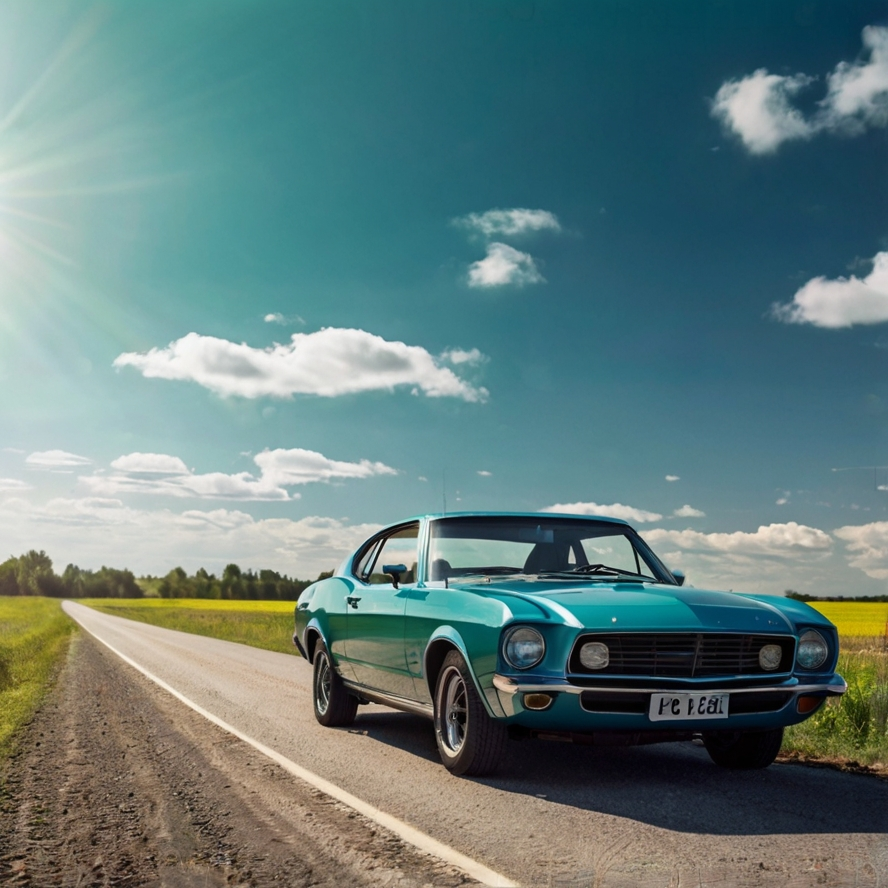
\includegraphics[width=1.8cm]{images/car.jpg}};    
\end{scope}

\node[s=1.8cm, draw, densely dashed, font=\footnotesize\ttfamily, align=left] (txt) at (ph-|d) {Question:\\[1mm]What color\\is the car?\\[1mm]Answer:};

% Arrows for group 1
\draw[->] (ph)--(c);
\draw[->] (txt)--(d);
\draw[->] (c)--(c|-b.south);
\draw[->] (d)--(d|-b.south);
\draw[->] (c|-b.north)--(c|-a.south);
\draw[->] (d|-a.north)--node[pos=1, above=1mm] {\scriptsize $<$EOS$>$} +(0,.5);
\draw[->] ($(d|-a.north)+(-1.05,0)$)--node[pos=1, above=1mm] {\scriptsize Blue} +(0,.5);

\node[below=.5cm] at ($(ph.south)!.5!(txt.south)$) {(a) \textbf{0-shot VQA}};

%---------------------- Second Group -------------------------
\node[draw, fill=myblue!15, w=8.2cm, h=.9cm, right=1cm of a] (a) {Self Attention Layers};

\node[draw, fill=gray!15, w=8.2cm, h=.4cm, below=.5cm of a] (b) {};

\node[draw, fill=mygreen!15, w=1.9cm, h=.9cm, anchor=north west] (c) at ($(b.south west)+(0,-.5)$) {Vision\\Encoder};

\node[draw, fill=mygreen!15, w=1.9cm, h=.9cm, right=2mm of c] (d) {Text\\Embedder};

\node[draw, fill=mygreen!15, w=1.9cm, h=.9cm, right=2mm of d] (e) {Vision\\Encoder};

\node[draw, fill=mygreen!15, w=1.9cm, h=.9cm, right=2mm of e] (f) {Text\\Embedder};


\foreach \i in {.25,.5,...,7.25}{
\begin{scope}[transform canvas={xshift=\i cm}]
\draw[rounded corners=.5mm] ($(b.north west)+(.1,0)$) -| ($(b.south west)+(0,0)$)--+(.1,0);    
\end{scope}
}

\begin{scope}
\node[below=.5cm of c, s=1.8cm] (ph) {};
\clip [rounded corners=.5mm] (ph.south west) rectangle (ph.north east);
\node[below=.5cm of c] (ph) {\includegraphics[width=1.8cm]{images/boeing.jpg}};    
\end{scope}

\node[s=1.8cm, draw, densely dashed, font=\footnotesize\ttfamily, align=left] (txt) at (ph-|d) {Q: Who\\invented\\this? A:\\ The Wright\\brothers};

\begin{scope}
\node[below=.5cm of e, s=1.8cm] (ph1) {};
\clip [rounded corners=.5mm] (ph1.south west) rectangle (ph1.north east);
\node[below=.5cm of e] (ph1) {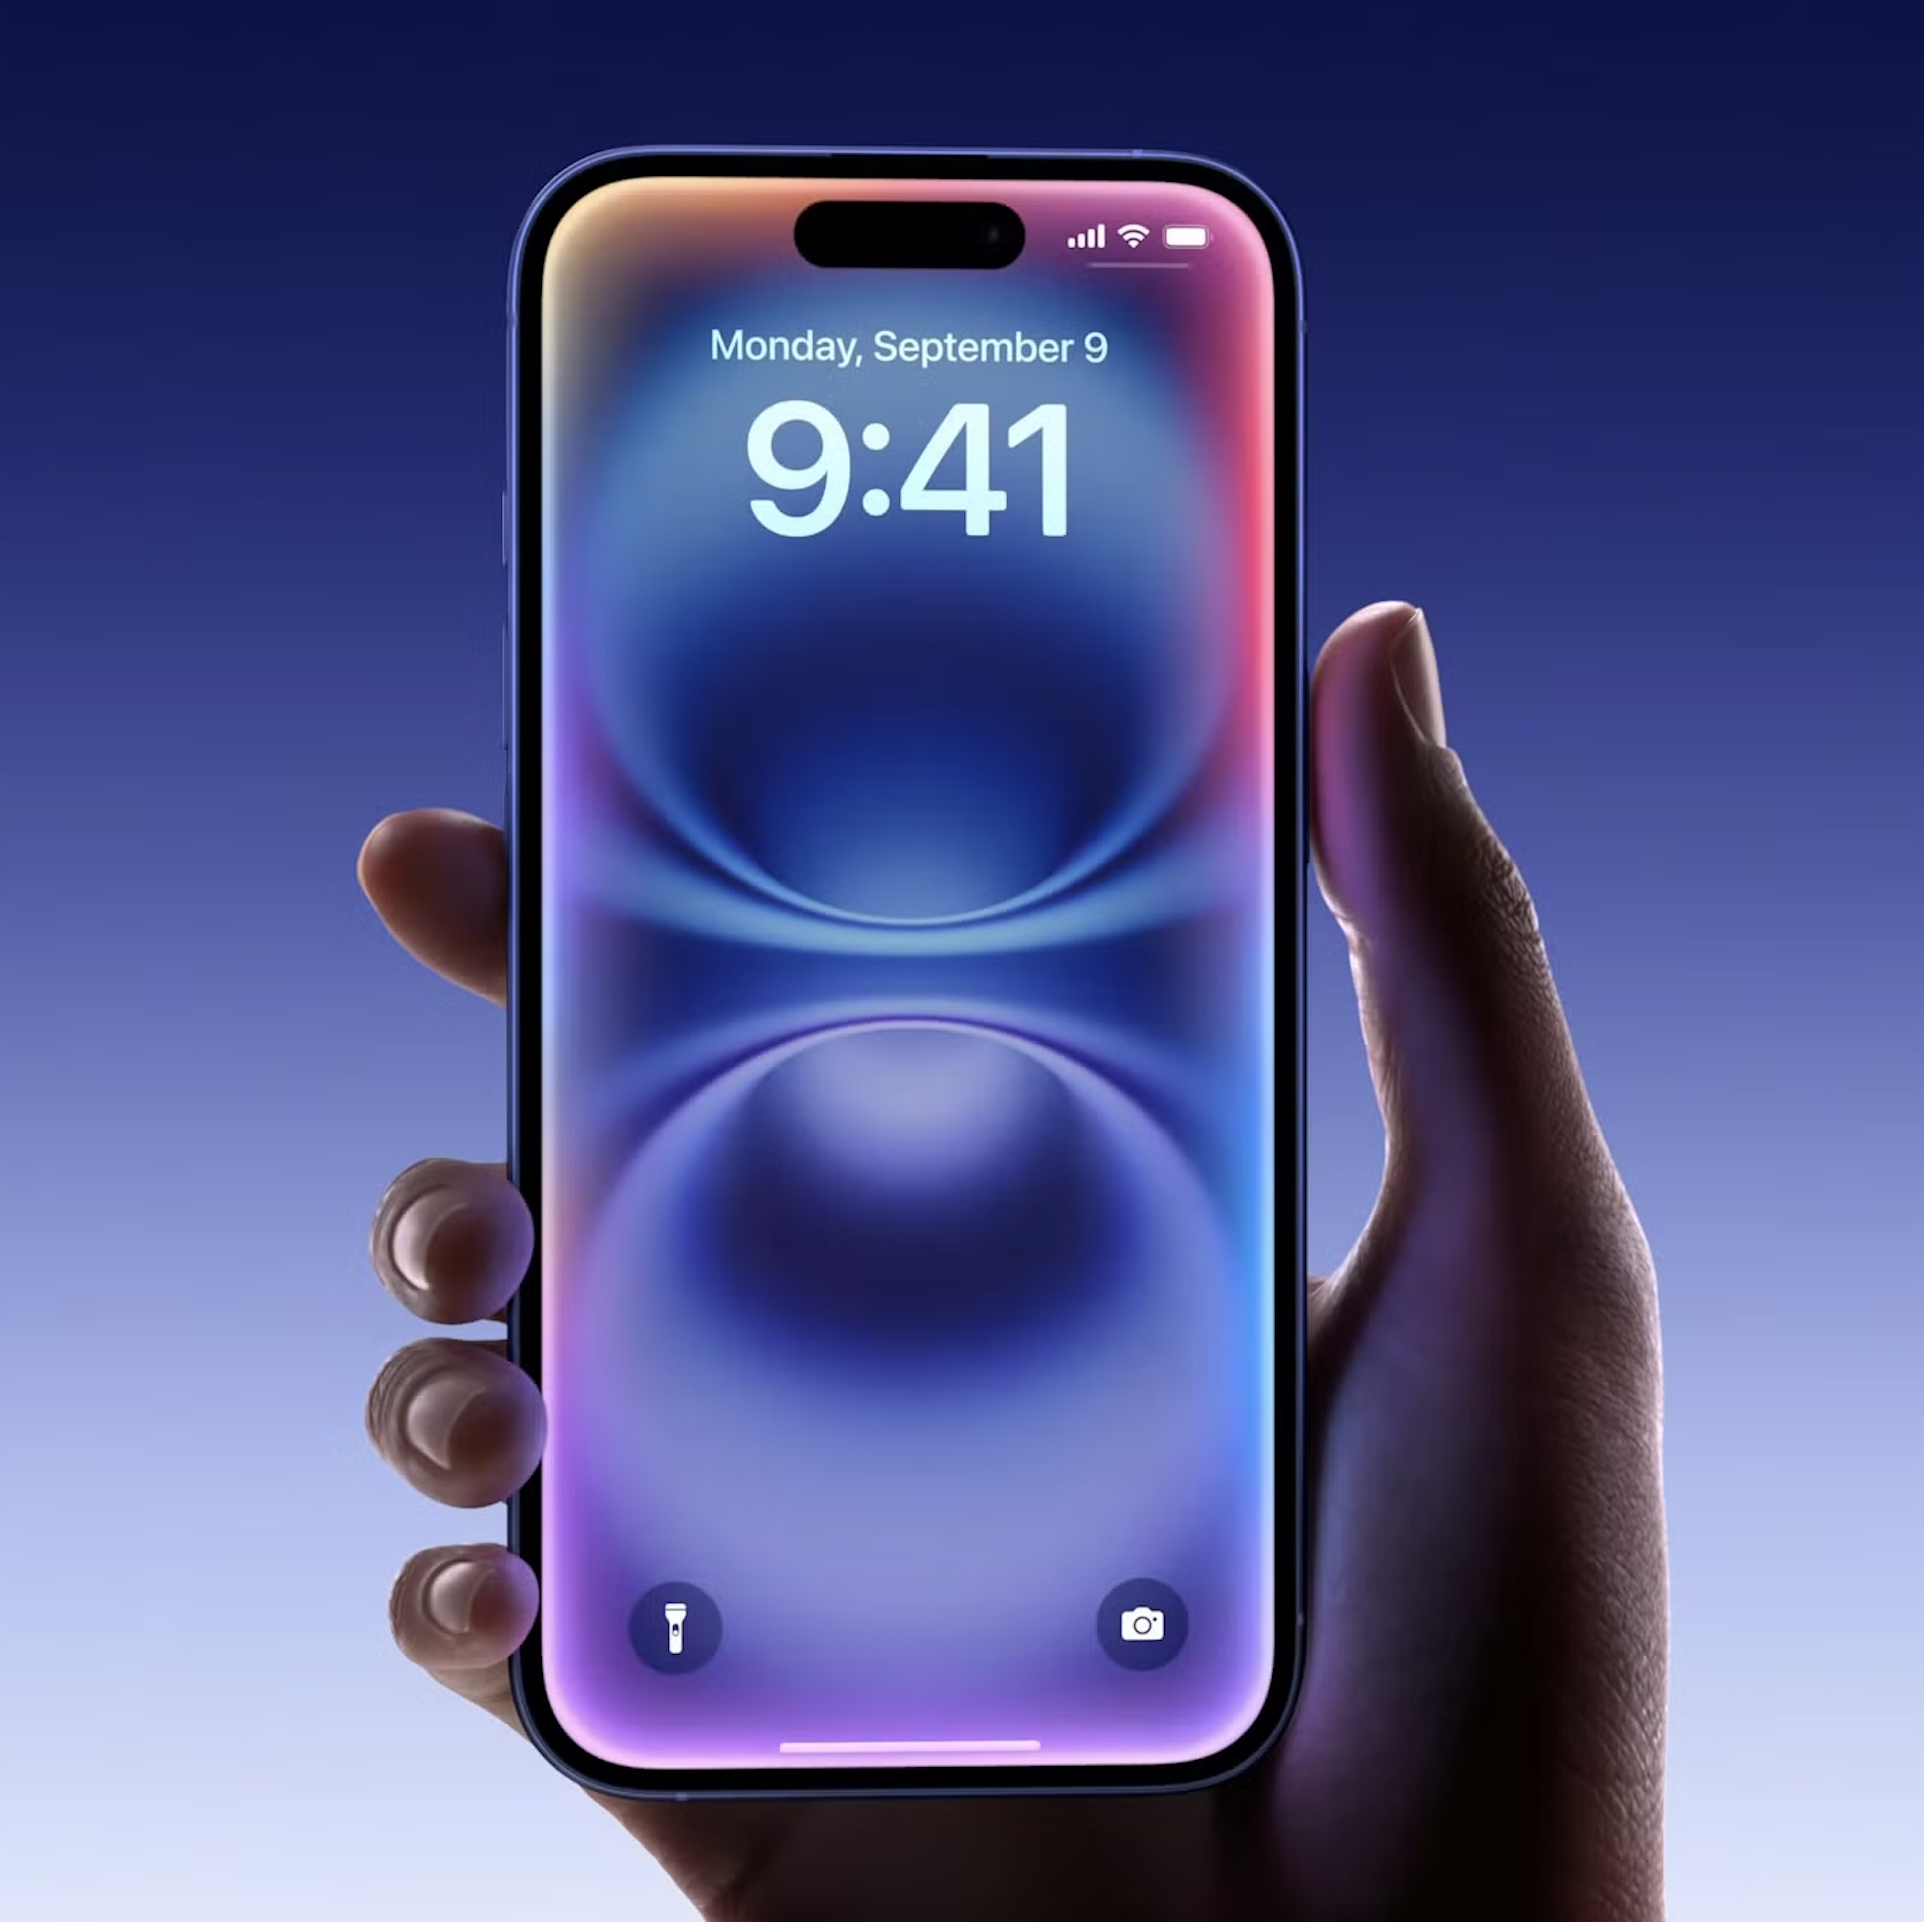
\includegraphics[width=1.8cm]{images/phone.jpg}};    
\end{scope}

\node[s=1.8cm, draw, densely dashed, font=\footnotesize\ttfamily, align=left] (txt1) at (ph1-|f) {Q: Who\\invented\\this? A:};

% Arrows for group 2
\draw[->] (ph)--(c);
\draw[->] (txt)--(d);
\draw[->] (c)--(c|-b.south);
\draw[->] (d)--(d|-b.south);
\draw[->] (ph1)--(e);
\draw[->] (txt1)--(f);
\draw[->] (e)--(e|-b.south);
\draw[->] (f)--(f|-b.south);
\draw[->] (c|-b.north)--(c|-a.south);

\draw[->] (f|-a.north)--node[pos=1, above=1mm] {\scriptsize $<$EOS$>$} +(0,.5);
\draw[->] ($(f|-a.north)+(-1.05,0)$)--node[pos=1, above=1mm] {\scriptsize .} +(0,.5);
\draw[->] (e|-a.north)--node[pos=1, above=1mm] {\scriptsize Jobs} +(0,.5);
\draw[->] ($(e|-a.north)+(-1.05,0)$)--node[pos=1, above=1mm] {\scriptsize Steve} +(0,.5);

\node[below=.5cm] at ($(txt.south)!.5!(ph1.south)$) {(b) \textbf{1-shot outside-knowledge VQA}};

%---------------------- Third Group -------------------------
\node[draw, fill=myblue!15, w=12.4cm, h=.9cm, below=7cm of a, xshift=-2.5cm] (a) {Self Attention Layers};
\node[draw, fill=gray!15, w=12.4cm, h=.4cm, below=.5cm of a] (b) {};
\node[draw, fill=mygreen!15, w=1.9cm, h=.9cm, anchor=north west] (c) at ($(b.south west)+(0,-.5)$) {Vision\\Encoder};
\node[draw, fill=mygreen!15, w=1.9cm, h=.9cm, right=2mm of c] (d) {Text\\Embedder};
\node[draw, fill=mygreen!15, w=1.9cm, h=.9cm, right=2mm of d] (e) {Vision\\Encoder};
\node[draw, fill=mygreen!15, w=1.9cm, h=.9cm, right=2mm of e] (f) {Text\\Embedder};
\node[draw, fill=mygreen!15, w=1.9cm, h=.9cm, right=2mm of f] (g) {Vision\\Encoder};
\node[draw, fill=mygreen!15, w=1.9cm, h=.9cm, right=2mm of g] (h) {Text\\Embedder};

\foreach \i in {.25,.5,...,11.5}{
    \begin{scope}[transform canvas={xshift=\i cm}]
        \draw[rounded corners=.5mm] ($(b.north west)+(.1,0)$) -| ($(b.south west)+(0,0)$)--+(.1,0);    
    \end{scope}
}

\begin{scope}
    \node[below=.5cm of c, s=1.8cm] (ph1) {};
    \clip [rounded corners=.5mm] (ph1.south west) rectangle (ph1.north east);
    \node[below=.5cm of c] (ph1) {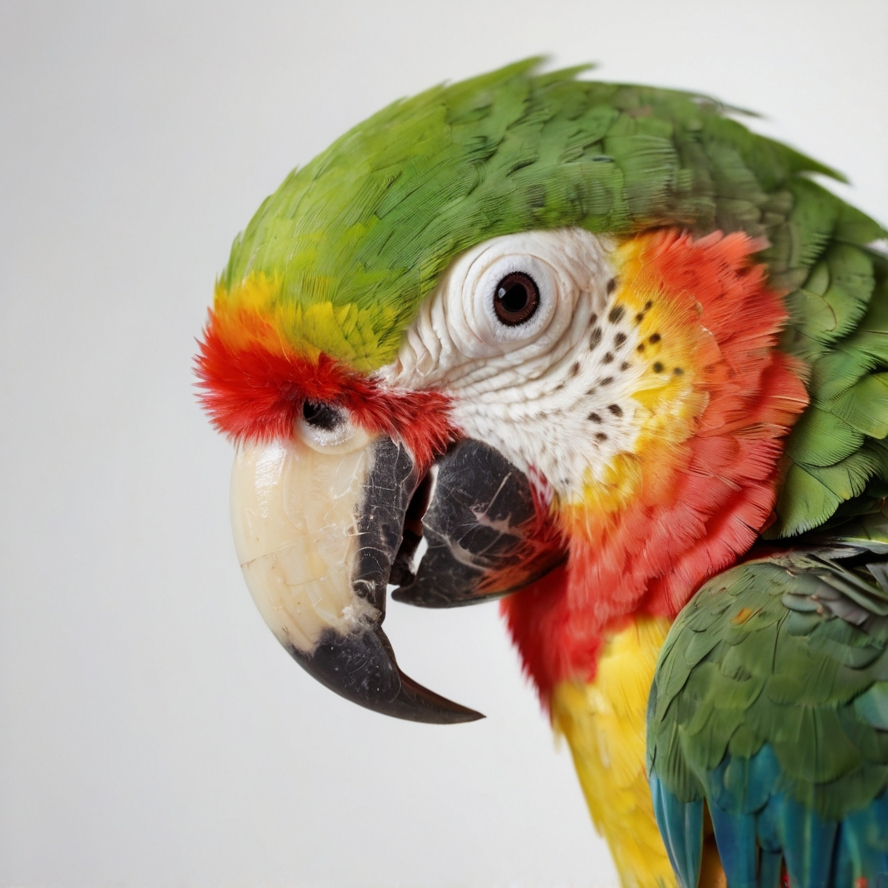
\includegraphics[width=1.8cm]{images/parrot4.jpg}};    
\end{scope}
\node[s=1.8cm, draw, densely dashed, font=\footnotesize\ttfamily, align=left] (txt1) at (ph1-|d) {This is a\\bird.};

\begin{scope}
    \node[below=.5cm of e, s=1.8cm] (ph2) {};
    \clip [rounded corners=.5mm] (ph2.south west) rectangle (ph2.north east);
    \node[below=.5cm of e] (ph2) {\includegraphics[width=1.8cm]{images/bird.jpg}};    
\end{scope}
\node[s=1.8cm, draw, densely dashed, font=\footnotesize\ttfamily, align=left] (txt2) at (ph2-|f) {This is a\\gull.};

\begin{scope}
    \node[below=.5cm of g, s=1.8cm] (ph3) {};
    \clip [rounded corners=.5mm] (ph3.south west) rectangle (ph3.north east);
    \node[below=.5cm of g] (ph3) {\includegraphics[width=1.8cm]{images/mosaic2/Dog5.jpg}};    
\end{scope}
\node[s=1.8cm, draw, densely dashed, font=\footnotesize\ttfamily, align=left] (txt3) at (ph3-|h) {Question:\\[1mm]What is\\this?\\[1mm]Answer:};

% Arrows for group 3
\draw[->] (ph1)--(c);
\draw[->] (txt1)--(d);
\draw[->] (c)--(c|-b.south);
\draw[->] (d)--(d|-b.south);
\draw[->] (ph2)--(e);
\draw[->] (txt2)--(f);
\draw[->] (e)--(e|-b.south);
\draw[->] (f)--(f|-b.south);
\draw[->] (ph3)--(g);
\draw[->] (txt3)--(h);
\draw[->] (g)--(g|-b.south);
\draw[->] (h)--(h|-b.south);
\draw[->] (c|-b.north)--(c|-a.south);

\draw[->] (h|-a.north)--node[pos=1, above=1mm] {\scriptsize $<$EOS$>$} +(0,.5);
\draw[->] ($(h|-a.north)+(-1.05,0)$)--node[pos=1, above=1mm] {\scriptsize .} +(0,.5);
\draw[->] (g|-a.north)--node[pos=1, above=1mm] {\scriptsize dog} +(0,.5);
\draw[->] ($(g|-a.north)+(-1.05,0)$)--node[pos=1, above=1mm] {\scriptsize a} +(0,.5);
\draw[->] (f|-a.north)--node[pos=1, above=1mm] {\scriptsize is} +(0,.5);
\draw[->] ($(f|-a.north)+(-1.05,0)$)--node[pos=1, above=1mm] {\scriptsize This} +(0,.5);

\node[below=.5cm] at ($(txt2.south)!.5!(ph2.south)$) {(c) \textbf{few-shot image classification}};
}

% }



\end{document}
